\documentclass{article}
\usepackage{amsmath}
\usepackage{amsthm}
\usepackage{amssymb}
\usepackage{enumerate}
\usepackage{graphicx}

\newenvironment{solution}{
    \par \textbf{Solution: } \quad \par
}{\par}

\begin{document}
    \title{Exercise 2.8}
    \author{Wang Yue from CS Elite Class}
    \date{\today}

    \maketitle

    \section*{Find the derivative of the function using the definition of derivative. State the domain of the function and the domain of its derivative.}

    \subsection*{26. $f(x) = x + \sqrt{x}$}

    \begin{solution}
        The domain of $f(x)$ is $[0, \infty)$.

        $$
        \begin{aligned}
            f'(x_0) &= \lim_{x \to x_0}\frac{f(x) - f(x_0)}{x - x_0} \\
            &= \lim_{x \to x_0}\frac{x - x_0 + \sqrt{x} - \sqrt{x_0}}{x - x_0} \\
            &= 1 + \lim_{x \to x_0}\frac{\sqrt{x} - \sqrt{x_0}}{x - x_0} \\
            &= 1 + \lim_{x \to x_0}\frac{1}{\sqrt{x} + \sqrt{x_0}} \\
            &= \frac{1}{2\sqrt{x_0}} + 1
        \end{aligned}
        $$

        $\therefore f'(x) = \frac{1}{2\sqrt{x}} + 1$, and the domain of $f'(x)$ is $(0, \infty)$.
    \end{solution}

    \subsection*{27. $g(x) = \sqrt{9 - x}$}

    \begin{solution}
        The domain of $g(x)$ is the solution set of $9 - x \geq 0$, which is $(-\infty, 9]$.

        $$
        \begin{aligned}
            g'(x_0) &= \lim_{x \to x_0}\frac{\sqrt{9 - x} - \sqrt{9 - x_0}}{x - x_0} \\
            &= \lim_{x \to x_0}\frac{9 - x - (9 - x_0)}{(x - x_0)(\sqrt{9 - x} + \sqrt{9 - x_0})} \\
            &= \lim_{x \to x_0}\frac{-1}{\sqrt{9 - x} + \sqrt{9 - x_0}} \\
            &= \frac{-1}{2\sqrt{9 - x_0}}
        \end{aligned}
        $$

        $\therefore g'(x) = \frac{-1}{2\sqrt{9 - x}}$, and the domain of $g'(x)$ is $(-\infty, 9)$.
    \end{solution}

    \subsection*{29. $G(t) = \frac{1 - 2t}{3 + t}$}

    \begin{solution}
        The domain of $G(t)$ is $\{ t \in R | t \not = -3 \}$.
        
        $G(t) = \frac{-6 - 2t + 7}{3 + t} = \frac{7}{t + 3} - 2$

        $$
        \begin{aligned}
            G'(t_0) &= \lim_{t \to t_0}\frac{\frac{7}{t + 3} - \frac{7}{t_0 + 3}}{t - t_0} \\
            &= 7 \lim_{t \to t_0}\frac{\frac{t_0 - t}{(t + 3)(t_0 + 3)}}{t - t_0} \\
            &= -7 \lim_{t \to t_0}\frac{1}{(t + 3)(t_0 + 3)} \\
            &= \frac{-7}{(t_0 + 3)^2}
        \end{aligned}
        $$

        $\therefore G'(t) = \frac{-7}{(t + 3)^2}$, the domain of which is also $(-\infty, -3) \cup (-3, \infty)$
    \end{solution}

    \subsection*{51. Let $f(x) = \sqrt[3]x$.}

    \begin{enumerate}[(a)]
        \item If $a \not = 0$, use Equation 2.7.5 to find $f'(a)$.

        \begin{solution}
            $$
            \begin{aligned}
                f'(a) &= \lim_{x \to a}\frac{f(x) - f(a)}{x - a} \\
                &= \lim_{x \to a}\frac{\sqrt[3]x - \sqrt[3]a}{x - a} \\
                &= \lim_{x \to a}\frac{(x^{\frac 1 3} - a^{\frac 1 3})(x^{\frac 2 3} + (ax)^{\frac 1 3} + a^{\frac 2 3})}{(x - a))(x^{\frac 2 3} + (ax)^{\frac 1 3} + a^{\frac 2 3})} \\
                &= \lim_{x \to a}\frac{1}{x^{\frac 2 3} + (ax)^{\frac 1 3} + a^{\frac 2 3}} \\
                &= \frac{1}{3(a)^{\frac 2 3}} \\
                &= \frac 1 3 a^{-\frac 2 3}
            \end{aligned}
            $$
        \end{solution}

        \item Show that $f'(0)$ does not exist.

        \begin{solution}
            $\because $ by problem (a), we can know the domain of $f'(a)$ is $(-\infty, 0) \cup (0, \infty)$
            
            $\therefore f'(0)$ has no definition, which means $f'(0)$ does not exist.
        \end{solution}

        \item Show that $y = \sqrt[3]x$ has a vertical tangent line at $(0,0)$.

        \begin{solution}
            $\because \lim_{x \to 0}f'(x) = \lim_{x \to 0}\frac{1}{3x^{\frac 2 3}} = \infty$

            $\therefore$ the tangent line of $f(x)$ as $x \to 0$ is vertical
            
            $\because \sqrt[3]0 = 0$

            $\therefore y = \sqrt[3]x$ has a vertical tangent line at $(0,0)$
        \end{solution}
    \end{enumerate}

    \section*{55.}

    \begin{enumerate}[(a)]
        \item Sketch the graph of the function $f(x) = x|x|$.

        \begin{solution}
            The graph of $f(x) = x|x|$ is below.

            \centering 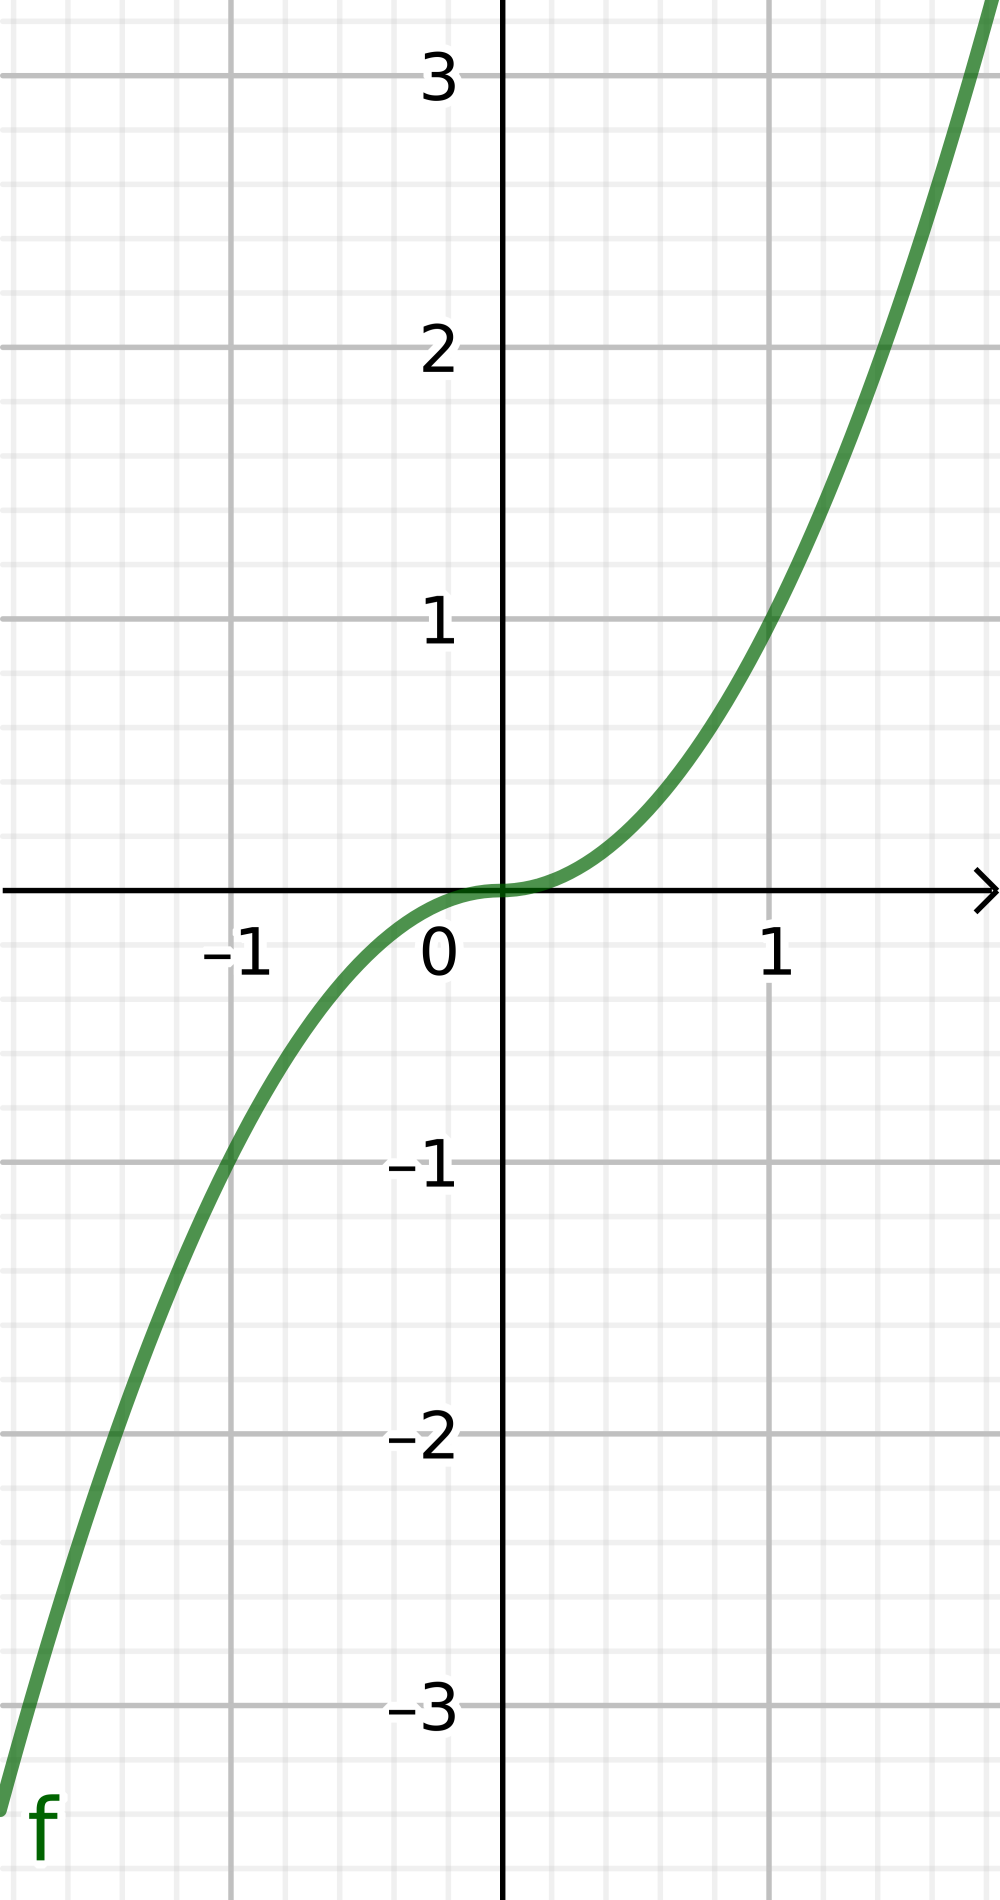
\includegraphics[scale=3.0]{geogebra-export.png}
        \end{solution}


        \item For what values of $x$ is $f$ differentiable?

        $\because f(x) = \left\{ \begin{array}{ll}
            x^2 & \textrm{if $x \geq 0$} \\
            -x^2 & \textrm{if $x < 0$} 
        \end{array} \right. $

        $\therefore f'(x) = \left\{ \begin{array}{ll}
            2x & \textrm{if $x \geq 0$} \\
            -2x & \textrm{if $x < 0$}
        \end{array} \right.$

        So obviously, for any value of $x$, $f(x)$ is differentiable.
        \item Find a formula for $f'$.

        By the problem (b), a formula for $f'$ can be $$f'(x) = 2|x|$$

    \end{enumerate}

    \section*{57. Prove each of the following.}

    \begin{enumerate}[(a)]
        \item The derivative of an even function is an odd function.

        \begin{proof}
            $\because f(x) = f(-x)$

            $\therefore$ taking derivative on the both side, we can get$$f'(x) = -f'(-x)$$

            which means $f'(x)$ is an odd function.
        \end{proof}

        \item The derivative of an odd function is an even function.

        \begin{proof}
            $\because f(x) = -f(-x)$

            $\therefore$ taking derivative on the both side, we can get $$f'(x) = f'(-x)$$

            which means $f'(x)$ is an even function.
        \end{proof}
    \end{enumerate}
\end{document}